\documentclass[11pt,a4paper]{article}
\usepackage{od}
\usepackage[utf8]{inputenc}
\usepackage[ngerman]{babel}

\pagestyle{headings}
\title{Cup des TRIZ-Summits – 2019/2020}

\author{Übersetzung des Textes ins Deutsche: Hans-Gert Gr\"abe, Leipzig}

\date{6. November 2019}

\newcommand{\video}{Die Clips sollten kurz sein (2 bis 5 Minuten). Es müsssen
  alle Autoren angegeben werden: Drehbuchautor, Kameramann, Cutter,
  Schauspieler usw.

Diese Arbeit zielt auf die Bildung von Lehrmaterial für die TRIZ-Ausbildung.

Auf der Website des TRIZ-Summit\footnote {\url
  {http://triz-summit.ru/en/contest/competition/video/}, \\ \url
  {https://www.youtube.com/channel/UCjMNOjboWRBQA72DJvaC7ew/featured}}
sind Videos vom letzten TRIZ Summit Cup veröffentlicht.}

\newcommand{\credentials}{Die Aufgaben des TRIZ Summit Cup 2018/2019 wurden
  vorbereitet von Rubin M.S., Rubina N.V., die Nominierung „Fantasie“ stammt
  von P.R. Amnuel.}

\newcommand{\melies}{
\begin{minipage}{.6\textwidth}
  \paragraph{1.}
  Der Gründer des Science-Fiction-Genres ist Franzose Filmemacher Georges
  Méliès. Jeder der über 500 Kurzfilme, Erstellt von Méliès zeichnet sich
  durch einen einzigartigen „Director's Style“ aus. Im Film „Besuch des Wracks
  des Kreuzers Maine“ (1897-1898) in der Folge „Divers at Work“ es war
  notwendig, ein klares Bild von Menschen zu zeigen, die unter Wasser
  arbeiten, und so weiter ein klares Bild von den Trümmern eines Kreuzers.
  Bilder unter Wasser zu dieser Zeit bereits fertig, aber sie waren eher
  exotisch, nicht gut genug sogar in sehr klarem Wasser. Schauen Sie sich zum
  Beispiel eines der ersten Fotos an Unter Wasser, hergestellt 1893 in
  Frankreich (einverstanden ist die Qualität nicht genug für die Folge des
  Films). Wie haben Sie es geschafft, eine Episode unter Wasser zu drehen?
  gute Qualität?
\end{minipage} \hfill
\begin{minipage}{.35\textwidth}
  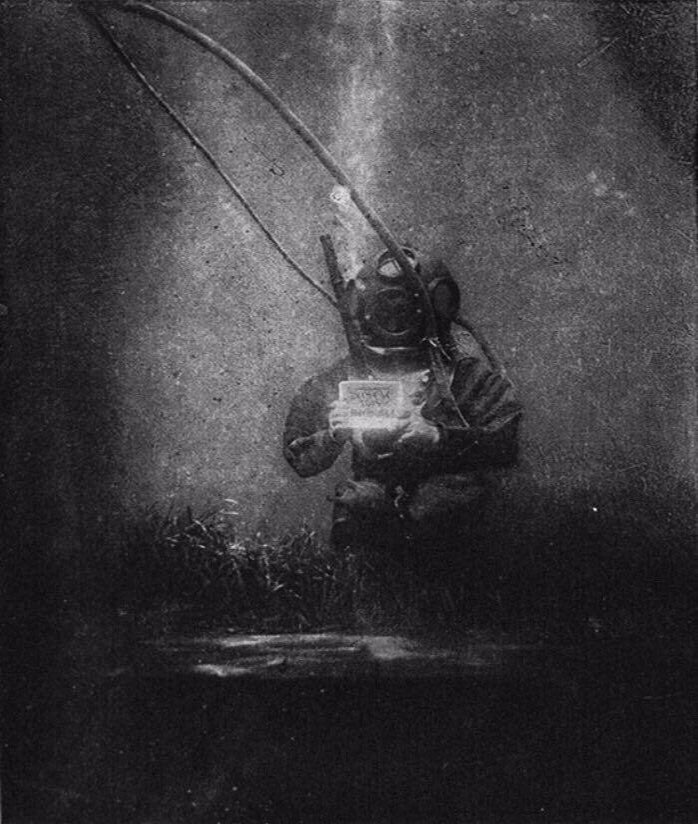
\includegraphics[width =\textwidth]{Bild-1.jpg}
\end{minipage}
\medskip

Der Film von J. Méliès „Im Reich der Feen“ mit ähnlicher Wirkung ist zu sehen
von Link: \url{https://www.youtube.com/watch?v=paM_BPyRT1o&t=542s}

Überraschenderweise verwendete er den gleichen Spezialeffekt in der
Filmgeschichte „Sadko“ Alexander Ptuschko im Jahr 1952 in Szenen auf dem
Meeresboden in der Nähe des Sea King.

Welche weiteren Spezialeffekte werden im Kino eingesetzt, um welche Probleme
zu lösen? Welche Widersprüche entstehen, durch welche Methoden werden sie
gelöst?
}

\newcommand{\hollywood}{\paragraph{2.}
In der Geschichte der Schaffung des größten Filmkonzerns der Welt - Hollywood
- gibt es Folgen, nicht bezogen auf künstlerisches Schaffen, nicht auf die
Erfindung neuer technischer Mittel für die Erstellung eines Films, aber mit
einem rein rechtlichen Problem. Bis zum Beginn des 20. Jahrhunderts Die
Person, die die Hauptpatente für Kinogeräte in Amerika besaß, erwies sich als
Thomas Edison (der gleiche Erfinder von Glühlampen). Jedoch die meisten
Filmemacher dieser Zeit waren die Haupteigentümer von Independent
Filmunternehmen. Außerdem arbeiteten sie alle an Geräten, die sie selbst
hatten verbessert und an die Umsetzung ihrer Ideen angepasst Filme. Aus diesen
Gründen hielten sie es nicht für notwendig, Edison zu bezahlen.  Interesse an
der Nutzung seiner Patente. Am 18. Dezember 1908 gab Edison bekannt Schaffung
von Motion Picture Patents Company (MPPC), die in die Geschichte des Kinos
eingegangen ist, wie der Edison Trust. Einige Filmfirmen haben sich der Firma
angeschlossen, die meisten jedoch wählte es, unabhängig zu bleiben. Der Tag
des 24. Dezember 1908, als sie eintrat Die Zuständigkeit des Trusts wurde in
der Geschichte des amerikanischen Kinos berühmt wie schwarze Weihnachten. Nach
den Regeln von Edison, Independent Filmfirmen mussten dem Trust enorme Summen
für das Rücktrittsrecht zahlen und einen Film zeigen. In New York unter dem
Vorwand der Patentverletzung Die Polizei schloss 500 der 800 Kinos. Welche
Entscheidung haben die Unabhängigen getroffen?  Filmfirmen, die nicht auf
Edison Trust angewiesen sind?

Kennen Sie Beispiele für kommerzielle Marketinglösungen, die beigetragen oder
behindert die Entwicklung des Kinos?
}

\newcommand{\kinogenres}{
\paragraph{1.}
Welche Filmgenres kennst du? Erstellen Sie eine Chronologie der Entstehung
verschiedener Genres Film. Markieren Sie die Muster der Darstellung
verschiedener Genres im Film, welche Ereignisse in der Geschichte das
Auftreten und die Entwicklung verschiedener Genres im Kino beeinflusst?
Identifizieren Sie in der Entwicklung von Kino-Genres Entwicklungslinien,
Muster bekannt in TRIZ? Welche Filmgenres mögen Sie mehr, warum?

\paragraph{2.}
Es gibt Menschen in der Geschichte des Kinos, deren Leistungen und Beiträge
zur Entwicklung des Kinos sehr wichtig sind bedeutend, aber die Namen sind
vergessen. Sammeln Sie Biografie-Informationen zu diesen Filmemacher. Welche
Aufgaben haben sie gelöst, welche Techniken haben sie angewendet? Wie geht es
Ihnen Denken Sie, welche Qualitäten der kreativen Persönlichkeit ihnen
geholfen haben, ihre Ziele zu erreichen?  Wenn eine Person ein bestimmtes
Problem löst, bleibt sie oft bei dem, was erreicht wurde, und nicht bei dem,
was erreicht wurde kann nichts mehr machen. Überraschenderweise ist die Firma
der Brüder Lumiere, ging in die Geschichte ein, als die Schöpfer des Kinos
aufhörten, Filme zu produzieren 1900, nur 5 Jahre nach der ersten
kommerziellen Vorführung von Filmen 28 Dezember 1895 - der Geburtstag des
Films. Was denkst du, könnte stören signifikante Ergebnisse in der Kreativität
zu erzielen?
}

\newcommand{\kinotools}{
\paragraph{1.}
Wählen Sie ein paar Tricks von Regisseuren, Kameraleuten, Toningenieure,
Drehbuchautoren (Schnitt, Pausen, Spezialeffekte, beschleunigte oder Zeitlupe
usw.) für alle Effekte in Film. Verwenden Sie diese Tricks in Ihren
Videos. Erweitern Sie Ihre Absicht im Detail Beschreibung des Videos. Ist es
möglich, diese Effekte mit TRIZ-Methoden zu verstärken?

\paragraph{2.}
Videos zur Geschichte der Fotografie, des Films und der Erfindungen, die in
gemacht wurden dieser Bereich.
}

\begin{document}
\maketitle

Die internationale öffentliche Organisation „TRIZ Developers Summit“ verkündet
die Durchführung des Wettbewerbs „TRIZ Summit 2020 Cup“ zur Theorie des
erfinderischen Problemlösens (TRIZ) für Schüler und Studenten. Am Wettbewerb
können sich Schüler und Studenten der TRIZ sowie Lehrer der TRIZ beteiligen.
Die Ergebnisse des Wettbewerbs werden nach Alterskategorien zusammengefasst:
8--10 Jahre; 11--14 Jahre; 15--17 Jahre; Studenten; Lehrer.

Die Gewinner des internationalen Wettbewerbs erhalten Diplome,
Teilnahmebescheinigungen und Erinnerungspreise. Der Wettbewerb dauert bis zum
22. März 2020. Alle Materialien sind elektronisch einzureichen. Die Adresse
für Korrespondenz und Einreichung von Wettbewerbsbeiträgen lautet
\url{TDS-2015@yandex.ru}.

Dies ist eine Kurzversion des Newsletters Nummer 1. Den genauen Text finden
Sie auf den
Seiten\footnote{\url{https://github.com/wumm-project/OpenDiscovery/tree/master/TRIZ-Cup/2020}}
des OpenDiscovery Projekts.

\credentials
\vfill
\tableofcontents
\vfill
\clearpage
\section{Kategorie 8--10 Jahre}

\subsection*{Nomination „Erfinden“}

\paragraph {1.}
Wenn du einen Zeichentrickfilm erstellen willst, sind mehrere Widersprüche zu
lösen:
\begin {itemize}
\item Die Zeichnungen, aus denen der Trickfilm zusammengestellt wird, sollen
  möglichst viele sein, damit die Bildübergänge glatt und ohne Sprünge sind,
  und sie sollten möglichst wenige sein, um die Zeit für die Erstellung eines
  Trickfilms zu verkürzen.
\item Zeichnungen, aus denen der Trickfilm besteht, sollten eine große Anzahl
  von Details enthalten, damit die Charaktere emotional sind, und sollten
  wenige Details enthalten, um die Erstellung des Trickfilms zu beschleunigen.
\item Die Kamera, die einzelne Zeichnungen aufzeichnet, muss stationär sein,
  damit das Bild klar ist und eine sich allmählich ändernde Position erfasst
  wird, und muss beweglich sein, um verschiedene Winkel und Räume zu erfassen,
  die das Objekt umgeben.
\end{itemize}
Wie wurden diese Widersprüche in verschiedenen Zeichentrickfilmtechniken
gelöst?

\paragraph{2.}
G.S. Altshuller schlug in dem Buch „Finde eine Idee“ eine Methode zum
Erstellen von Geschichten für Trickfilme (oder Märchen) vor, die als
„Geschichten mit Widersprüchen“ bezeichnet werden kann.  Der Algorithmus zum
Erstellen eines solchen Märchens (Handlung für den Trickfilm) lautet wie
folgt:

\begin{enumerate}
\item Wähle Personen oder ein Objekt märchenhaften Charakters aus.
\item Stelle kurz die Umgebung der Personen vor.
\item Wende die Technik des Fantasierens an (vergrößern, verkleinern, zum
  Gegenteil übergehen, beleben, kombinieren\footnote{In der Ausschreibung:
    „fantastisches Binom“ -- eine Kombinationstechnik, die auf Gianni Rodari
    zurückgeht} usw.). Formuliere eine märchenhafte \textsc{Idee}.
\item Formuliere die Anti-Idee und den Widerspruch. Baue eine Handlung auf
  basierend auf Lösungen dieses Widerspruchs.
\item Führe Einschränkungen ein oder erstelle einen neuen Widerspruch auf der
  Basis der Widerspruchslösung des vorigen Punkts -- entwickle damit die
  Handlung weiter.
\item Es entsteht eine sehr dynamische Handlung.
\end{enumerate}
Denke dir mit diesem Algorithmus eine Handlung für einen Trickfilm aus.

\subsection*{Nomination „Fantasie“}

\paragraph{1.}
1974 schrieb der amerikanische Science-Fiction-Autor James Tiptree die
Geschichte „Das Mädchen, das eingesperrt wurde“ (The Girl Who Was Plugged In).
Es gibt folgende Episode in der Geschichte: Der Film wird mit Lasern auf
Wolken über der Stadt projiziert, und alle Einwohner, die nach oben schauen,
können dem Film zuschauen. Nun ist dies fast keine Fiktion -- Lasershows auf
den Wolken sind beliebt geworden. Dies sind jedoch noch keine Filme.  Überlege
dir eine neue, fantastische Möglichkeit, Filme zu demonstrieren.

\paragraph{2.}
Der sowjetische Science-Fiction-Autor Nikolai Vasilenko beschrieb in der
Geschichte „Der krumme Spiegel“ (1977) einen fantastischen Spiegel: Wenn ein
Mensch in ihn hineinschaut, dann sieht er nicht sein Spiegelbild, sondern
einen kleinen Film, in dem ihm das Wesen seiner Person als Bild eines Tieres
gezeigt wird. Denke dir auf dieser Idee eine fantastische Geschichte aus, aber
ändere die Idee mit einer der Fantasietechniken.

\subsection*{Nominierung „TRIZ Tools“}

\paragraph{1.}
Aus welchen Elementen besteht die Werkbank zur Erstellung von Trickfilmen? Wie
hängen sie zusammen?  Welche Funktionen erfüllt jedes Element?  Aus welchen
Materialien können Charaktere für den Trickfilm hergestellt werden?  Denke dir
deinen eigenen Charakter für den Trickfilm aus und eine kleine Geschichte über
ihn.

\paragraph{2.}
Stelle ein Archiv mit Beispielen für die Verwendung von Fantasietechniken in
Trickfilmen und Märchenfilmen zusammen. Analysiere das Archiv. Welche
Techniken werden häufiger zum Erstellen typischer Charaktere oder Bilder
verwendet (wie z.B. entsteht das Bild eines neugierigen, boshaften und mutigen
Pinocchio\footnote{im Original: „Buratino“}: die lange (vergrößerte) Nase
fordert direkt dazu auf, „die Nase in die Angelegenheiten anderer Leute zu
stecken“; Das „belebte“ Holzstück „sinkt nicht im Wasser und brennt nicht im
Feuer“). Vergleiche, wie in verschiedenen Trickfilmen (Märchenfilmen) ähnliche
Bilder erzeugt werden (gute und böse Zauberer, starke Helden, schöne
Prinzessinnen, launische Prinzessinnen usw.). Was ist dein
Lieblings-Trickfilm? Welche Sequnzen in diesem Trikfilm magst du und werden
dort Fantasietechniken verwendet?

\subsection*{Nomination „Forschung“}
Stelle ein Archiv mit Trickfilmen über Erfinder (oder Wissenschaftler) und
ihre Erfindungen (Entdeckungen) zusammen. Analysiere das Archiv. Welche
Aufgaben lösen die Helden der Filme?  Mit welchen Techniken werden die
Probleme gelöst? Wie werden die gefundenen Lösungen (Entdeckungen) im Leben
der Menschen angewendet?

%--- bis hierher durchgesehen

\subsection*{Nominierung „TRIZ Videos“}
\begin{enumerate}
\item Wähle ein paar Tricks, die von Regisseuren verwendet werden, Operatoren,
  Tontechniker, Drehbuchautoren (Schnitt, Pausen, Spezialeffekte, schnelle
  oder langsame Bewegung usw.) für alle Effekte im Kino. Verwenden Sie diese
  Tricks in Ihren Videos. Erweitern Sie Ihre Angaben Design in der
  Beschreibung des Videos. Ist es möglich, diese Effekte mit Methoden zu
  verbessern?  TRIZ?
\item Videos zur Geschichte der Fotografie, des Films und der Erfindungen, die
  es gab in diesem Bereich gemacht.
\end{enumerate}
\video

\clearpage
\section{Kategorie 11-14 Jahre}

\subsection*{Invention nomination}

\paragraph{1.}
1909 filmte der amerikanische Filmemacher David Griffith einen Stummen
Kurzfilm (Dauer 7 Minuten) „Die abgeschiedene
Villa“\footnote{\url{https://www.youtube.com/watch?time_continue=13&v=5RdbnyNYAv8}}.
Das Actionfilm über den Versuch, eine reiche abgelegene Villa auszurauben.
Wahrscheinlich Dies ist der allererste Film im Thriller-Genre (Actionfilm, der
provoziert) Zuschauer Spannung und Aufregung). Der Film präsentiert drei
Sichtweisen:
\begin{itemize}
  \item Familie in der Heimat und vor dem Angriff fliehen;
  \item Banditen, die ein wohlhabendes Haus angreifen;
  \item das Familienoberhaupt und die Bullen erscheinen im „letzten Moment“.
\end{itemize}
Griffith hatte die Aufgabe (in 7 Minuten) die Handlung dieser Geschichte zu
zeigen, Eindringen in das Haus, Angst vor der Hausherrin und ihren drei
Töchtern, Körperverletzung und, Die Hauptsache ist die Erlösung. Vor der
Gründung von Solitary Villa waren Filme enthalten Handlungen, die ein Ereignis
abdecken und die Abfolge der Aktionen widerspiegeln Charaktere mit chronischer
Zuverlässigkeit (Zeit im Kino fiel mit Zeit zusammen) Ereignisse im
Leben). Wie man in kurzer Zeit verschiedene Handlungsstränge zeigt und den
Eindruck (Spannung) des Publikums stärken? Was für ein Filmgerät zuerst
angewendet D. Griffith? Was andere Filmtechniken erfanden David Griffith und
welche Effekte haben sie erzeugt? Wählen Sie eine Aufgabe oder mehrere
Aufgaben, die D. Griffith gelöst und analysiert hat das folgende Schema:
Widersprüche formulieren, RBIs, Ressourcen auflisten, In der Aufgabe stehen
Methoden zur Lösung von Widersprüchen zur Verfügung, die genutzt werden können
in dieser Aufgabe. Welche Filmtechniken kennen Sie, um welche zu entscheiden?
Aufgaben bewerben sie sich?

\paragraph{2.}
Wenn Sie einen Trickfilm erstellen, müssen Sie mehrere Widersprüche auflösen:
\begin{itemize}
\item der Zeichnungen, aus denen der Trickfilm besteht, sollte so groß wie
  möglich sein Das Bild war glatt, ohne Sprünge, und die Zeichnungen sollten
  so gut wie möglich sein weniger, um den Prozess des Erstellens eines
  Trickfilms in der Zeit zu reduzieren;
\item Zeichnungen, aus denen der Trickfilm besteht, sollten die größte Anzahl
  enthalten Details, damit die Charaktere emotional sind, und sollten mit den
  wenigsten sein die Menge an Details, um die Erstellung des Trickfilms zu
  beschleunigen;
\item muss die Kamera, die einzelne Zeichnungen aufzeichnet, stationär sein,
  damit Das Bild war klar und nahm eine sich allmählich ändernde Position ein
  Objekte und müssen beweglich sein, um verschiedene Winkel und Volumen zu
  erfassen Raum, der das Objekt umgibt.
\end{itemize}
Wie wurden diese Widersprüche in verschiedenen Zeichentechniken gelöst?

\subsection*{Fantasy Nomination}

\paragraph{1.}
Der amerikanische Science-Fiction-Autor Thomas Sherred beschrieb den Film
gefilmt mit einer zeitmaschine. Überlegen Sie sich eine fantastische Art zu
produzieren Filme. Wie werden sie in Zukunft Filme machen?

\paragraph{2.}
In der Geschichte von Pavel Amnuel „Der fliegende Adler“ (1970) erfindet der
Dramatiker Das Stück schreibt nicht den Text, wie er jetzt ist, sondern
erzeugt ein Video, das sich vorstellt als ob das Stück bereits inszeniert
wäre. Er braucht keine Schauspieler, er stellt sich die Figuren selbst vor,
ihr Spiel und Verhalten. Erstelle eine Geschichte, die auf dieser Idee
basiert, aber ändere sie sie mit etwas Fantasietechnik.

\subsection*{Nominierung „TRIZ Tools“}

Beschreiben Sie das technologische Prinzip des Films. Aus welchen Teilen
besteht CINEMA?  Wie interagieren diese Teile miteinander, um eine filmische
Wirkung zu erzielen?  Wirkung? Welche Effekte (physikalisch, chemisch,
physiologisch) werden genutzt?  beim Erstellen und Anzeigen eines Films? Wie
hat die Wahrnehmung und das Denken der Menschen über die Jahrzehnte des Kinos?
Was denkst du welche Auswirkungen wird in Zukunft im Kino eingesetzt?

\subsection*{Forschungsnominierung}

\paragraph{1.}
Welche Filmgenres kennst du? Erstellen Sie eine Chronologie der Entstehung
verschiedener Genres Film. Ist es möglich, die Entwicklungslinien am Beispiel
von Genres im Kino zu veranschaulichen?  in TRIZ bekannte Systeme
(z. B. Dynamisierung, Mono-Bi-Poly-Koagulation, Übergang zu einem Supersystem,
Übergang zu einer Mikroebene). Welche Filmgenres bevorzugen Sie?  wie warum?

\paragraph{2.}
1927 fand die Uraufführung des Films „Singer
Jazz“\footnote{\url{https://my.mail.ru/mail/wikki0508/video/5622/29304.html}}
- Der erste Tonfilm in der Geschichte des Kinos. Der moderne Betrachter ist
schon Es ist schwer, sich einen Film ohne Worte und Soundeffekte
vorzustellen. Allerdings nicht alle Die Filmemacher akzeptierten diese
revolutionäre Veränderung sofort. „Stille, Die Zweidimensionalität und
Gleichförmigkeit des Films sind keine Mängel, sondern „konstruktiv Essenz.
Kinokunst muss nicht wie neu überwunden werden Ausdrucksmittel werden seine
weitere Verbesserung nur behindern“ - So schrieb über die Merkmale der Kunst
des Kinos Yu. Tynyanov in den 30er Jahren. Versuchen Sie es beweisen Sie die
gegensätzlichen Standpunkte: Sprechen Sie zuerst auf der Seite Gegner der
Einführung von Ton in das Kino, und dann auf der Seite der Befürworter davon
Technologie. Welche neuen Soundeffekte erscheinen Ihrer Meinung nach in Filmen
in die Zukunft?

\subsection*{Nominierung „TRIZ Videos“}

\paragraph{1.}
Wählen Sie ein paar Tricks von Regisseuren, Kameraleuten, Toningenieure,
Drehbuchautoren (Schnitt, Pausen, Spezialeffekte, beschleunigte oder Zeitlupe
usw.), um Filmeffekte zu erhalten.  Verwenden Sie diese Tricks in Ihren
Videos. Erweitern Sie Ihre Absicht im Detail Beschreibung des Videos. Ist es
möglich, diese Effekte mit TRIZ-Methoden zu verstärken?

\paragraph{2.}
Videos zur Geschichte der Fotografie, des Films und der Erfindungen, die in
gemacht wurden dieser Bereich.

\video
\clearpage

\section{Kategorie 15-17 Jahre}

\subsection*{Invention nomination}

\melies

\hollywood

\subsection*{Fantasy Nomination}

\paragraph{1.}
In dem Roman des amerikanischen Science-Fiction-Schriftstellers Philip Dick
„Träumen Androids von Elektrikern?“ beschreibt ein Gerät, mit dem eine Gruppe
von Menschen in die Gefühle der Auserwählten eindringen kann Mann, um die Welt
so zu fühlen, wie er sich fühlt. So können Sie einen Film machen und das
Publikum Sie werden alles spüren, was der Schauspieler während der
Dreharbeiten gefühlt hat. Komm mit einem neuen eine fantastische Idee, indem
Dicks Idee mit einem „Grundriss“ geändert wird G. S. Altshuller.

\paragraph{2.}
Alexander Belyaev beschrieb im Roman „Lord of the World“ (1929) das
„Gedankentheater“, in welche schauspieler nicht auf der bühne spielen, sie
präsentieren ihr spiel nur gedanklich und der zuschauer „fängt“ diese gedanken
ein und „sieht“ geistig die aufführung. Komm mit eine fantastische Geschichte
über das Filmen eines solchen „Gedankenfilms“, der die Idee von Belyaev mit
verändert mit einer der fantasierenden Techniken.

\subsection*{Nominierung „TRIZ Tools“}

Bei der Entwicklung technischer Systeme können mehrere Entwicklungslinien
unterschieden werden, zum Beispiel „Mono-Bi-Poly-Koagulation“;
„Dynamisierung“; „Leere“; „Übergang auf die Mikroebene ”; „Persönlich -
persönlich-kollektiv - kollektiv.“ Sammeln ein Aktenschrank mit Beispielen für
diese Filmentwicklungslinien oder fotos. Denken Sie daran, dass sowohl Kino
als auch Fotografie Kunst und Technologie sind.  Produktion und kommerzielles
Produkt (Kinos, Werbung, verwandte Service usw.).

\subsection*{Forschungsnominierung}
\kinogenres

\subsection*{Nominierung „TRIZ Videos“}
\kinotools 
\video
\clearpage

\section{Kategorie Studenten}

\subsection*{Invention nomination}

\melies

\hollywood

\subsection*{Fantasy Nomination}

\paragraph{1.}
In den fantastischen Geschichten des japanischen Schriftstellers Kobo Abe
„Totaloscope“ und Der italienische Schriftsteller Lino Aldani „Oniofilm“
(beide Erzählungen erscheinen in 1965) werden Filme beschrieben, die mit
voller Wirkung von Anwesenheit und Rückseite gedreht wurden Kommunikation mit
dem Betrachter. Ändern Sie diese Idee mit Fantasy-Techniken, mit nicht einer
Technik, sondern mehreren. Beschreiben Sie das Ergebnis.

\paragraph{2.}
US-amerikanische Science-Fiction Frank Herbert im Weltraumepos „Dune“ (1965)
beschrieben, wie einer der Charaktere das Verhalten anderer Benutzer steuert
spezielle Intonationen der Stimme. Gleichzeitig geht es der kontrollierten
Person gut versteht, kann aber nichts tun: er ist gezwungen zu gehorchen. Komm
mit die Handlung für einen Abenteuerfilm der Zukunft, basierend auf Herberts
Idee, aber Ändern Sie es, während sich die Handlung unter Verwendung von
Fantasietechniken entwickelt.

\subsection*{Nominierung „TRIZ Tools“}

Die Entwicklungsgesetze technischer Systeme bilden die Grundlage der TRIZ. Es
gibt mehrere mögliche Klassifikationen dieser Gesetze. Wir bieten Ihnen einen
davon an.
\begin{center}
  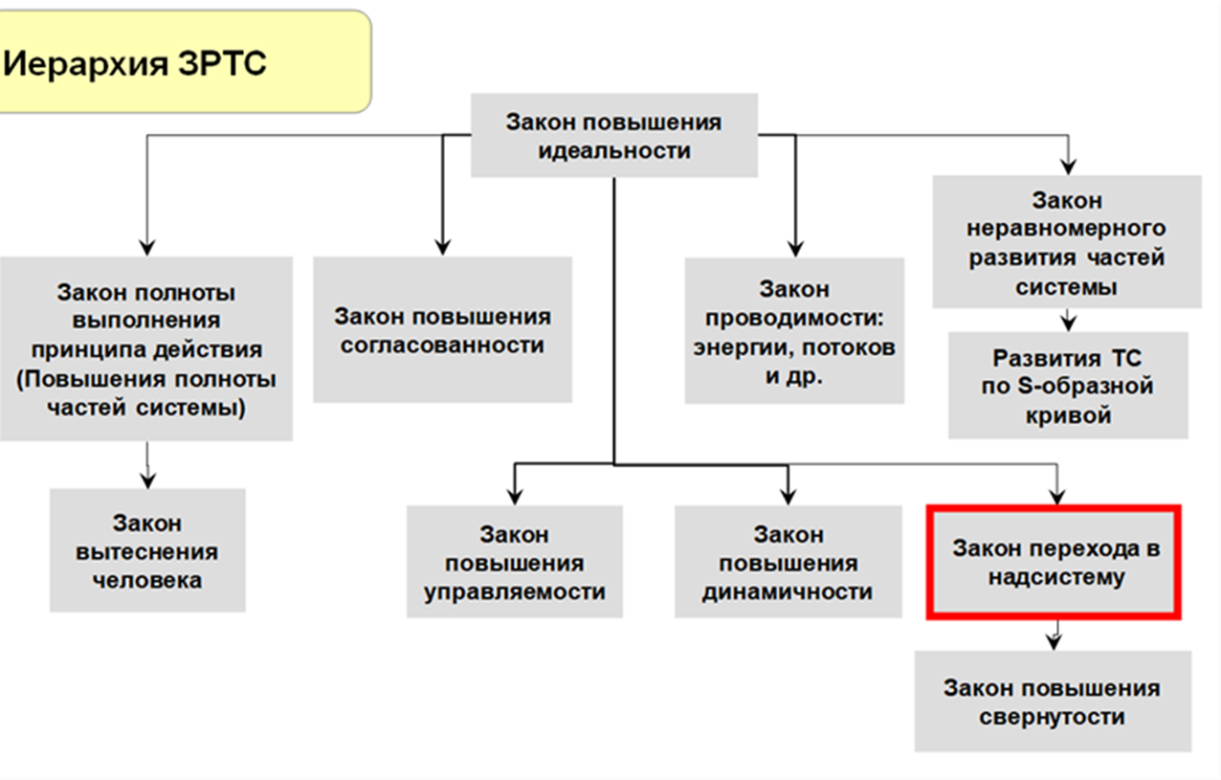
\includegraphics[width=.9\textwidth]{oE4yUs.png}
\end{center}
Analysieren Sie die Entwicklungsstadien des Kinos mithilfe des Rechtssystems
Entwicklung technischer Systeme. Wie in Anbetracht der von Ihnen
identifizierten Trends Können Sie die weitere Entwicklung des Kinos
vorhersagen?

\subsection*{Forschungsnominierung}
\kinogenres
\subsection*{Nominierung „TRIZ Videos“}
\kinotools

\video


\end{document}
